% CDSM method paper. Author fields are intentionally blank at the user's request.
% Unmodified official acmart/pvldb styles; no compressed margins or body fonts.
\documentclass[sigconf,nonacm]{acmart}
\usepackage{pvldb}
\usepackage{amsmath,tabularx,array,xurl}
\usepackage{algorithm}
\usepackage{algpseudocode}
\settopmatter{printacmref=false}
\graphicspath{{figures/}}
\newcolumntype{Y}{>{\raggedright\arraybackslash}X}
\newcommand{\cdsm}{\textsc{CDSM}}
\newcommand{\severe}{\mathrm{Severe}}
\newcommand{\recall}{\mathrm{Recall}}
\newcommand{\dc}{\mathrm{DC}}
% Generated only from the completed latest server control wave.
\newcommand{\rTwoQpsC}{$-3.28\%$ to $-2.58\%$}
\newcommand{\rTwoQpsDev}{$-7.28\%$ to $-3.70\%$}
\newcommand{\rTwoQpsFrontier}{$+28.21\%$ to $+33.44\%$}
\newcommand{\rTwoQpsSixteen}{$-8.83\%$ to $-7.00\%$}
\newcommand{\rTwoDevCluster}{$+0.112$ percentage points, with a descriptive query-cluster 95\% interval of $[+0.069,+0.157]$}

\hypersetup{pdftitle={CDSM: Budgeted Multi-Entry Search for Reducing Severe Recall Failures},pdfauthor={},pdfsubject={Method paper with frozen T2I, LAION and WebVid evaluation}}
\begin{document}
\title{CDSM: Budgeted Multi-Entry Search for Reducing Severe Recall Failures}
\begin{abstract}
Graph-based approximate nearest-neighbor search can achieve high average recall while missing most true neighbors for some queries. We present CDSM, which uses bounded exploration from alternative entrances to redirect a continuing main search. Short local searches, called scouts, share scores and traversal progress, then return unfinished executable work to the main frontier. Every stage consumes one query budget. On four T2I graphs at exactly 10,240 distance evaluations per query, the original four-scout policy reduces severe recall failures by 44--72\% and raises mean Recall@10 by 0.214--0.398 percentage points over direct continuation, with QPS changes of \rTwoQpsC{}. It also raises mean recall over all tested 1/4/8/16-entry shared-queue controls at this budget, while larger entrance counts offer competing tail-quality tradeoffs. Starting scouts from the existing frontier does not reproduce its quality gains. At measured points giving continuation 10\% more work, CDSM still has higher recall, fewer severe failures, and 7.50--8.30\% higher throughput. Neighboring scout depths and separate query cohorts support its T2I applicability; frozen LAION and WebVid transfer lowers mean recall. CDSM improves limited-budget search on the demonstrated workloads without rebuilding the graph or predicting query recall.
\end{abstract}
\maketitle
\pagestyle{plain}
% Publication metadata and the author block are deliberately not fabricated.
% Fill the official \vldbtopmatter fields when preparing an actual submission.
\section{Introduction}\label{sec:intro}
HNSW uses upper layers to find an entrance and bottom-layer search to refine candidates~\cite{hnsw}. Even after construction, the search policy determines which opportunities receive computation before a query ends. Improving that allocation can benefit an existing index without rebuilding its edges.

High average recall can hide severe misses. On one T2I graph, direct continuation achieves 99.06\% mean Recall@10, yet 32 of 8,000 queries retrieve fewer than five true top-ten neighbors, and ten retrieve none. We study whether a fixed computation allowance can better serve these queries while preserving average quality and accounting for execution time.

Continuation gives all remaining computation to the existing frontier. Additional entrances create opportunities but immediately compete with a mature queue. Independent searches let routes develop, yet merging only their answers discards unfinished expansions. How can another route develop within a limited allowance while preserving paid progress?

\cdsm{} pauses the main route, runs short local searches called \emph{scouts}, and feeds their unfinished work back into the main frontier. A scout uses its own result threshold, allowing a route to develop before competing with the main route's answers. Shared scores, discovery marks, and adjacency cursors preserve progress. Reintegrated candidates can redirect subsequent main expansions toward answers that neither the original continuation nor the scouts had scored. A global collector retains answers; frontier feedback preserves further discovery opportunities.

The primary policy F uses a fixed entrance table and up to four scouts of 400 distance evaluations each, without a learned rescue predictor. Local queues, shared visitation, resumed search, and inter-path feedback have precedents, including iQAN~\cite{iqan}. Our contribution is how additional exploration is initiated, bounded, and integrated with an already progressed search under one budget.

On four T2I graphs at exactly 10,240 distance evaluations, F reduces severe failures by 44--72\% and raises mean recall by 0.214--0.398 percentage points over continuation, with QPS changes of \rTwoQpsC{}. A same-framework grid compares one, four, eight, and sixteen entrances, including development selection, and scouts launched from the existing main frontier. F raises mean recall over every MEP size at this budget; its severe-failure advantage is less uniform, revealing competing uses of the same computation. Native Faiss, adaptive stopping, and a same-graph FANNG reconstruction provide further quality--cost context.

At measured points, F at 10,240 evaluations also has higher mean recall, fewer severe failures, and 7.50--8.30\% higher throughput than C at 11,264. Thus another 10\% of continuation work does not eliminate the advantage there; this does not imply dominance at every budget.

The T2I reference configuration is tested across query cohorts, graph constructions, budgets, and nearby scout depths. Fixed transfer to LAION and WebVid lowers mean recall despite some rescues; paid selection also supplies tradeoffs. These boundaries accompany the method's positive results.

The paper contributes (1) a budgeted search method that redirects main-search expansion through bounded local exploration and shared unfinished state; (2) evidence of improved average and severe-failure quality on T2I, including equal-work and stronger-continuation controls with measured throughput; and (3) full-cohort ablations, execution interventions, and frozen transfer that establish the mechanism and the observed applicability of the method.

\section{Problem and Resource Model}\label{sec:problem}
Let $G=(V,E)$ be a fixed graph over stored vectors, $q$ a query, and $N_k(q)$ the exact nearest-neighbor set. We return $A_k(q)$ and evaluate
\[
 \recall@k(q)=\frac{|A_k(q)\cap N_k(q)|}{k}.
\]
We use $k=10$. A \emph{severe failure} has fewer than five true neighbors, and a \emph{zero-recall failure} has none. A rescue crosses from severe to non-severe; a harm crosses in the opposite direction. These are outcomes computed from exact ground truth, not signals available to the search policy.

The controlled resource is actual query--vector distance evaluation. All new scores---including upper descent, entrance selection, scouts, and final continuation---consume one common allowance $B_q$. A cached score does not execute another distance computation and incurs no additional unit, although its lookup and queue processing still take CPU time. Equal distance work therefore does not imply equal latency. We report both resources.

Two contracts are evaluated separately. Under an \emph{absolute cap}, $B_q=B$ for every query. Under the \emph{additional-allowance contract}, $B_q=P_q+E$, where $P_q$ is the actual initial-stage expenditure and $E$ is fixed. The initial stage can stop early, so $P_q+E$ is not generally $6{,}400+E$. An execution may finish below its cap if all recoverable work is exhausted; the strict comparisons reported here verify equality of actual work query by query instead of inferring it from matching configured caps.

A \emph{frontier} comprises discovered candidates with unfinished expansion work. It includes waiting active or deferred candidates and a current node whose adjacency list has been only partly processed. An empty active queue alone does not imply an empty recoverable frontier. Storing only the best $k$ answers cannot represent these continuation opportunities.

\section{CDSM}
\label{sec:method}

CDSM's primary policy F runs up to four local \emph{scouts}, each capped
at 400 new distance evaluations, then continues from their reintegrated
state. Local thresholds let routes develop before competing with the
main answers. We describe squared L2, where smaller distances are better.

\begin{figure*}[t]
\centering
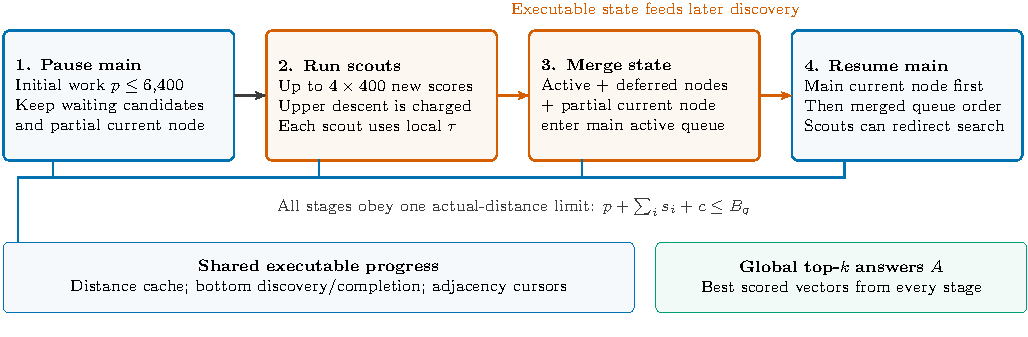
\includegraphics[width=\textwidth]{method-feedback.pdf}
\Description{Four stages show a paused main search, bounded local scouts, reintegration of active, deferred and partly expanded nodes, and main continuation. All stages share scores and traversal progress; the answer collector is distinct from executable frontier state.}
\caption{CDSM-F's execution organization (conceptual, not a measured trajectory). Scouts return executable bottom-layer work to the main frontier. The suspended main current node resumes first; the merged candidates then compete by query distance, potentially redirecting later expansions. All new distance evaluations share the query limit $B_q$.}
\label{fig:method}
\end{figure*}

\paragraph{Shared state.}
One workspace shares a distance cache, global top-$k$ collector $A$,
bottom-layer discovery/completion marks, and each opened node's next-neighbor
cursor. Discovery means entering bottom traversal, distinct from being
scored during upper descent. Main frontier $M$ retains active and deferred
candidates plus an optional partially expanded current node. Each scout
has a separate empty local frontier and top-$k$ set, while sharing the
workspace. Every first physical score updates $A$: an upper-layer
discovery can improve the answer without subsequent bottom exploration.

\paragraph{Initial search and entrances.}
The main search descends from the graph's ordinary HNSW entry point.
It spends at most $P_{\max}=6400$ evaluations, including descent.
Between node expansions, it can stop when the closest pending candidate's
squared distance is at least $(1+\gamma)^2 \tau_A$, where $\gamma=0.075$
and $\tau_A$ is the current global $k$th distance.
This condition applies only after $A$ contains $k$ answers.
The search retains its queues and any incomplete adjacency cursor.
Let $p$ denote its actual evaluation count.

A graph-specific table supplies up to 64 distinct upper-layer nodes in a
query-independent, sampled order; imported graphs retain their saved table.
Appendix~\ref{app:execution} gives the exact construction.
The order is not a learned utility ranking.
At each scout, F takes the first table node not previously used as a scout
entrance and not already discovered by bottom-layer traversal.

\paragraph{Local exploration.}
For current distance count $d_c$, a scout receives the boundary
$L=\min(B_q,d_c+400)$.
Its upper descent begins at the selected node's highest layer and charges
all new distances against $L$.
After descent, the local top-$k$ set $T$ is cleared.
If budget remains and the endpoint is not bottom-layer discovered, the
endpoint seeds the local frontier and $T$.
Thus upper-layer scores can improve $A$ without prematurely tightening
the scout's local threshold.

The scout resumes a partially expanded node before selecting another one.
For an undiscovered neighbor, it reads the pre-update threshold
$\tau=T_k$, or $\infty$ while $T$ is not full, and obtains its cached
or newly computed distance $d$.
It marks the neighbor discovered.
If $d<\tau$, it inserts the neighbor into its active queue and updates $T$;
otherwise it retains the neighbor in its deferred queue.
Between expansions, deferred candidates with distance below the current
$\tau$ become active, and completed nodes are discarded.
The scout pauses when no eligible active candidate remains, when the
best active distance exceeds $\tau$, or when $L$ is reached.
A candidate farther than the global $k$th answer can still be locally
promising and expose neighbors absent from the main route.

\paragraph{Reintegration and continuation.}
F inserts each scout's active, deferred, and unfinished current work into
the main active queue, retaining shared cursors, then clears the local
frontier for reuse. Scouts are not independently scheduled afterward.
Continuation resumes the main suspended current node first, then orders
merged candidates by distance. It skips completed nodes, admits new
bottom discoveries without a local threshold, and disables initial
distance stopping. Thus locally rejected work remains available for
further discovery; reintegration retains more than scout answers.

\paragraph{Budgeted execution.}
Algorithm~\ref{alg:cdsm} summarizes the stages.
The total limit is either a fixed $B_q$, known before initialization,
or $B_q=p+E$ under an additional-allowance contract.
With a fixed limit, the initial stage is also capped by $B_q$.

\begin{algorithm}[t]
\small
\begin{algorithmic}[1]
\Require Query $q$, graph $G$, entrance table $\mathcal E$, budget contract
\State Initialize shared workspace $W$, answers $A$, frontier $M$
\State $b_0\gets\min(6400,B)$ if absolute; otherwise $6400$
\State Descend and run main search under $b_0$, $\gamma=0.075$
\State Preserve $M$; $p\gets d_c$ \Comment{actual distance count}
\State $B_q\gets B$ if absolute; otherwise $p+E$
\For{$i=1,\ldots,4$ while $d_c<B_q$}
  \State $e\gets$ first unused, bottom-undiscovered node in $\mathcal E$
  \If{no such $e$} \State \textbf{break} \EndIf
  \State Mark $e$ used; $L\gets\min(B_q,d_c+400)$
  \State $v\gets\Call{UpperDescend}{e,L,W}$
  \State Clear local frontier $S$ and local top-$k$ set $T$
  \If{$d_c<L$ and $v$ is bottom-undiscovered}
    \State Seed $v$ into $S,T$; mark $v$ bottom-discovered
    \State $\Call{LocalExplore}{S,T,L,W}$ using the local rules
  \EndIf
  \State Insert $S$.active, $S$.deferred, $S$.current into $M$.active
  \State Retain shared cursors and $M$.current; clear $S$
\EndFor
\State Resume $M$.current, then merged frontier under $B_q$
\State Use unrestricted admission and no distance stopping
\State \Return $A$
\end{algorithmic}
\caption{CDSM-F. Upper descent and local exploration check their limit before each new score. Final continuation stops at the limit or when recoverable work is exhausted.}
\label{alg:cdsm}
\end{algorithm}

Traversal routines check the relevant boundary before every new scoring
operation. Cache hits do not spend a physical evaluation.
If scout $i$ spends $s_i$ and final continuation spends $c$, then
$p+\sum_i s_i+c\leq B_q$.
Early scout stops leave more budget for continuation; they do not enlarge
another scout's 400-evaluation limit.
F neither adds filler work nor guarantees that every graph permits
exhausting $B_q$.
Equal actual evaluations therefore require measurement, and do not imply
equal queue work or latency.

Paid-selection and scheduling extensions are evaluated separately in
Section~\ref{sec:family}; their selection work uses the same query budget.

\paragraph{Reference configuration and parameter meaning.}
Table~\ref{tab:parameters} fixes the retained development settings for T2I
and transfer, without claiming optimality or a newly preregistered selection.
We test other graphs, allowances, and neighboring scout depths; dimension-
or size-based parameter scaling remains unvalidated.

\begin{table}[t]
\centering\small
\caption{Frozen F parameters and query-dependent quantities.}
\label{tab:parameters}
\begin{tabularx}{\columnwidth}{@{}llY@{}}
\toprule
Symbol & Value & Meaning \\
\midrule
$k$ & 10 & Returned answers; local threshold size \\
$P_{\max}$ & 6,400 & Initial upper and bottom scoring limit \\
$\gamma$ & 0.075 & Initial stopping slack; disabled in final phase \\
$m,s$ & 4, 400 & Maximum scouts and new distances per scout \\
$|\mathcal E|$ & $\leq64$ & Distinct upper-layer entrance table \\
$p$ & Measured & Actual initial expenditure for this query \\
$B_q$ & $B$ or $p+E$ & Total allowed new distances \\
$\tau_A,\tau$ & Dynamic & Global and scout-local $k$th distances \\
\bottomrule
\end{tabularx}
\end{table}

\begin{table*}[t]
\centering\small
\caption{Search organization. C and MEP are controlled policies; FANNG is our same-graph search reconstruction. iQAN is a literature comparison, not a measured baseline in this study.}
\label{tab:semantics}
\begin{tabularx}{\textwidth}{@{}lYYY@{}}
\toprule
Method & Where exploration starts & Allocation and coordination & What determines subsequent expansion \\
\midrule
C & Retained main-search state & All remaining budget to one route & Existing frontier and adjacency cursors \\
MEP-$m$ & Up to $m$ backup upper entrances & Paid descent endpoints enter a shared queue; $m=1,4,8,16$ & Common queue order; no private scout interval \\
FRONTIER & Up to four pending main-frontier candidates & F's local scouts, with cached roots and shared progress & Unfinished scout work returns to the main frontier \\
FANNG search & Common upper-descent endpoint & One edge at a time under the distance budget & Query-prioritized source and remaining-edge cursor \\
iQAN~\cite{iqan} & Multiple candidates from the search pool & Local queues, staged path expansion, adaptive synchronization & Local paths feed candidates back into global search \\
CDSM-F & Backup entrances after a main-search prefix & Up to four local scouts; 400 new distances each & Active, deferred, and current scout work joins the main frontier with shared cursors \\
\bottomrule
\end{tabularx}
\end{table*}


\section{Experimental Design}\label{sec:design}
\paragraph{Graphs and scoring.}
We use one million 200-dimensional T2I vectors~\cite{t2i}, one Faiss graph (M32, construction ef 200), and three imported Lucene 9.12 graphs (M16, construction ef 100; seeds 42, 777, 1234). Lucene builds share original insertion order, single-threaded writes, and serial merges, testing construction randomness rather than insertion order. Import preserves edges, neighbor order, and vector identities; controlled methods share each graph. LAION-CLIP1M and WebVid1M transfer uses three graphs per dataset (M16, construction ef 100) and 512-dimensional vectors~\cite{laion,webvid}; Appendix~\ref{app:details} specifies their subsets and provenance.

Server runs use normalized float32 vectors, squared L2, and matching exact top-ten truth. Earlier Java validation uses Lucene COSINE and its own truth. Neither tests unnormalized inner product; the four T2I graphs remain one dataset.

\paragraph{Controls.}
\textbf{C} spends all remaining work on the original frontier, sharing F's scoring, caching, and outputs; it is not native HNSW. \textbf{MEP-$m$}, $m\in\{1,4,8,16\}$, attempts eligible entrances from the same table, charges descent to the total budget, and injects completed endpoints into the common queue without private scouts. Unlike the older MEP control, descent has no separate 400-evaluation limit. Visitation can change later entrance eligibility.

\textbf{FRONTIER} freezes up to four distinct, incomplete main-frontier candidates by distance and ID, excluding the suspended current node. Each starts a 400-evaluation scout with F's threshold, shared progress, reintegration, and continuation. Taking over a root preserves its cursor; completed roots are skipped without replacement. Root scores are cached; selection and queue maintenance count toward time. This specified control explores existing candidates and is not native iQAN.

\textbf{FANNG} reconstructs Algorithm~3's distance-budgeted backtracking search~\cite{fanng}: one edge at a time from a query-prioritized source, retaining its cursor. It preserves HNSW bottom edges, sorts each adjacency offline by edge length and ID, and disables pruning ($T=\infty$). Common upper descent replaces centroid initialization; every scored candidate can enter the global collector. An independent reference checks paths, outputs, and accounting. This is a search reconstruction, not native FANNG construction or its optimized system.

\textbf{Native Faiss}, uncapped \textbf{ABS}, and \textbf{ABS\_CAP} supply quality--time context~\cite{faiss,abs}. Native retains its own stopping policy. ABS and its hard-cap variant use audited shared-backend search implementations. Their selected operating points do not assert equal distance work. The subsequent restriction of uncapped ABS to $\gamma<0.06$ is disclosed; it does not change F's internal 0.075 initial stopping rule.

\paragraph{Cohorts and execution.}
Main and transfer runs use 8,000 quality queries and an 800-query timing subset. Serial, single-threaded timing uses CPU 22 of an Intel Xeon Gold 5117 at 2.00\,GHz. Latest controlled, family, and transfer points have two 32-query warmup passes and five rounds in randomized task order. QPS is the inverse mean of per-query median latency; p95/p99 are quantiles of these medians, not raw service latencies. Earlier native/ABS timing instead uses ten-query warmup and median round-level QPS. These times, and local Java/MEP times, remain within their own waves. Section~\ref{sec:newqueries} identifies earlier unused-query cohorts.

\paragraph{Budget and inference.}
Absolute caps are 8,192, 10,240 (primary), and 12,800. The latest control wave freezes F and evaluates all four MEP sizes plus FRONTIER. Before evaluation, a separate, historically used 1,000-query development set selects \textbf{MEP-DEV} per graph and cap by greatest mean recall, then fewest severe failures, then smallest $m$. Selection is never per query. At 10,240 we additionally vary F's per-scout limit to 200 and 800, returning unused work to continuation. No policy is retuned on these results.

Family allowances are 3,200 (primary) and 6,400. For these, a frozen manifest supplies $P_q$ to all methods; FANNG receives the same $B_q$, not C's bottom-layer prefix state. Manifest generation is excluded from every timer. Absolute caps require no query-dependent budget generation.

We report paired rescues and harms and exact two-sided McNemar tests. The latest primary family compares F with MEP-4, MEP-DEV, and FRONTIER on four graphs at 10,240: twelve tests with Holm correction, retaining duplicated MEP choices conservatively. Paired 95\% intervals use 5,000 bootstrap draws; four-graph summaries cluster by query ID. These intervals are descriptive, not simultaneous. Earlier families remain separate: four F/FANNG tests; twenty adjacent extension tests at $E=3{,}200$; and three/fifteen tests for each transfer dataset. Historical queries and repeated graph--query events do not supply independent fresh-query confirmation. QPS point differences within 1.5\% are practically negligible by our stated tolerance, not statistically equivalent.

\section{Evaluation}\label{sec:results}
\subsection{Same graph, same actual distance work}\label{sec:fixed}
Figure~\ref{fig:budget} compares C, F, development-selected MEP, and FRONTIER across four T2I graphs and three budgets. Table~\ref{tab:fixed} includes every MEP size at the primary budget. All 736,000 evaluation records, including the two neighboring depths, spend exactly their cap; shared initial states are checked per query. The 192,000 C/F records reproduce archived scoring-sequence hashes, answers, and counters, adding no independent C/F evidence.

\begin{figure*}[t]
\centering
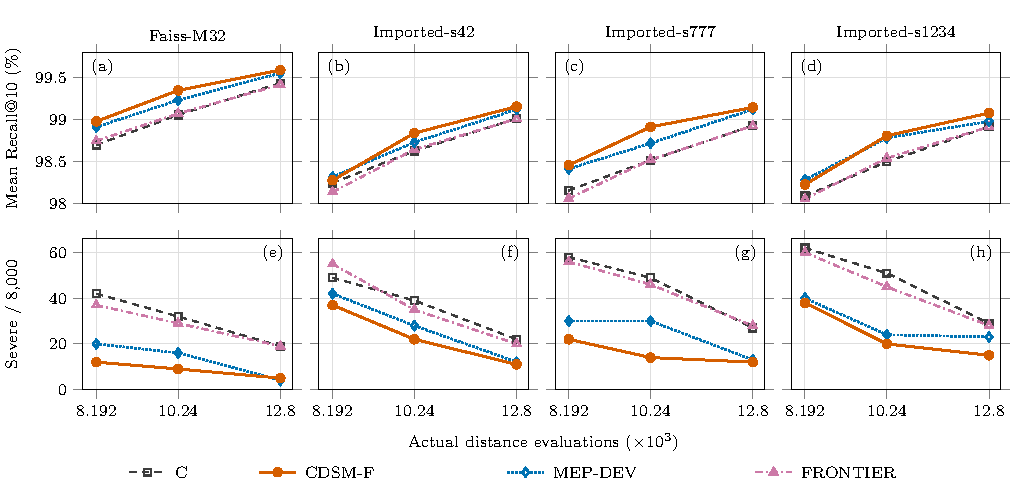
\includegraphics[width=\textwidth]{t2i-budget.pdf}
\Description{Eight panels show mean recall and severe-failure counts at three equal distance budgets on four T2I graphs for C, CDSM-F, development-selected MEP, and scouts launched from the existing frontier.}
\caption{Budget response on four fixed T2I graphs, sharing 8,000 query identities. Every query spends exactly the indicated distance count. MEP-DEV selects one entrance count per graph and budget on disjoint development queries; the chosen count may change between points. Lines connect measured points, not confidence bounds. Table~\ref{tab:fixed} exposes the complete primary MEP grid.}
\label{fig:budget}
\end{figure*}
\begin{table*}[t]
\centering
\caption{T2I at exactly 10,240 evaluations per query. Each cell is mean Recall@10 (\%) / severe failures out of 8,000 / QPS. All times are remeasured together in the latest control wave. F (200/800) changes only the per-scout limit; F (400) is the frozen original.}
\label{tab:fixed}
\small
\begin{tabular}{@{}lrrrr@{}}
\toprule
Policy & Faiss M32 & Imported 42 & Imported 777 & Imported 1234 \\
\midrule
C & 99.0587 / 32 / 281.0 & 98.6275 / 39 / 265.1 & 98.5175 / 49 / 265.4 & 98.4988 / 51 / 263.6 \\
F (400) & 99.3513 / 9 / 271.8 & 98.8413 / 22 / 257.3 & 98.9150 / 14 / 257.8 & 98.8100 / 20 / 256.8 \\
MEP-1 & 99.1262 / 27 / 281.3 & 98.6912 / 32 / 264.5 & 98.5600 / 44 / 265.2 & 98.5825 / 45 / 264.8 \\
MEP-4 & 99.2300 / 17 / 284.5 & 98.7313 / 28 / 267.2 & 98.7200 / 30 / 268.0 & 98.6412 / 38 / 267.9 \\
MEP-8 & 99.2362 / 16 / 289.0 & 98.7362 / 26 / 270.7 & 98.7738 / 25 / 270.6 & 98.7263 / 30 / 271.2 \\
MEP-16 & 99.2788 / 6 / 298.1 & 98.8062 / 18 / 276.7 & 98.8675 / 16 / 277.4 & 98.7837 / 24 / 277.0 \\
FRONTIER & 99.0750 / 29 / 203.7 & 98.6463 / 35 / 199.6 & 98.5237 / 46 / 199.0 & 98.5413 / 45 / 200.3 \\
F (200) & 99.3313 / 11 / 280.7 & 98.8150 / 23 / 263.0 & 98.8263 / 21 / 263.8 & 98.7775 / 24 / 263.4 \\
F (800) & 99.3637 / 8 / 266.2 & 98.8825 / 20 / 254.9 & 98.9087 / 14 / 255.7 & 98.8075 / 20 / 254.4 \\
\bottomrule
\end{tabular}
\end{table*}


At 10,240, F increases mean recall over C by 0.214--0.398 percentage points and reduces severe failures by 44--72\%. Faiss M32's severe risk falls from $32/8{,}000=0.400\%$ to $9/8{,}000=0.1125\%$. C/F rescues/harms are 26/3, 19/2, 35/0, and 33/2; all four pass the earlier 28-test correction. The latest same-wave QPS differences are \rTwoQpsC{}. Queue work and reintegration have real time costs despite equal scoring work.

\paragraph{Beyond shared-queue multiple entrances.}
At the primary budget, F has higher mean recall than every MEP size on all four graphs. MEP-DEV selects $m=8,4,4,16$ in graph order. Relative to those choices, F gains 0.115/0.110/0.195/0.02625 percentage points and changes severe counts from 16/28/30/24 to 9/22/14/20. The four-graph mean gain is \rTwoDevCluster{}; this interval preserves the same query across graphs and is not multiplicity-adjusted. F's QPS differences from MEP-DEV are \rTwoQpsDev{}.

\begin{table*}[t]
\centering
\caption{Primary severe-failure comparisons at 10,240. Entries are rescues/harms when replacing the control with F, followed by the exact McNemar $p$ value after Holm correction across twelve tests. DEV gives the development-selected MEP entrance count; duplicated MEP choices are not independent evidence.}
\label{tab:closest}
\small
\begin{tabular}{@{}lrrrr@{}}
\toprule
Graph & DEV $m$ & MEP-4 to F & MEP-DEV to F & FRONTIER to F \\
\midrule
Faiss M32 & 8 & 11/3 (0.287) & 12/5 (0.438) & 23/3 ($7.04\!\times\!10^{-4}$) \\
Imported 42 & 4 & 8/2 (0.438) & 8/2 (0.438) & 15/2 (0.014) \\
Imported 777 & 4 & 16/0 ($3.05\!\times\!10^{-4}$) & 16/0 ($3.05\!\times\!10^{-4}$) & 33/1 ($4.89\!\times\!10^{-8}$) \\
Imported 1234 & 16 & 20/2 ($8.48\!\times\!10^{-4}$) & 13/9 (0.523) & 30/5 ($2.46\!\times\!10^{-4}$) \\
\bottomrule
\end{tabular}
\end{table*}


Table~\ref{tab:closest} limits the severe-failure claim: F beats MEP-4 after Holm correction on seeds 777/1234, but beats MEP-DEV significantly only on seed 777. Moreover, MEP-16 has fewer severe failures than F on Faiss M32 (6 versus 9) and seed 42 (18 versus 22), while having lower mean recall on both. Giving extra entrances a bounded local interval therefore improves average quality here, but does not uniformly dominate a larger entrance count on the tail endpoint.

\paragraph{Starting scouts from the current frontier.}
F raises mean recall over FRONTIER by 0.195--0.391 percentage points. Severe counts change from 29/35/46/45 to 9/22/14/20; all four primary tests pass Holm correction. QPS differences are \rTwoQpsFrontier{}; FRONTIER builds a sorted candidate set, so this time result does not represent an optimized frontier scheduler. Existing candidates do not reproduce F's quality gains here. Actual local expenditure and later eligibility also differ: this is a complete-policy comparison, not isolated proof that upper entrances alone cause the gain.

Budget changes reveal further tradeoffs. At 8,192, MEP-DEV has higher mean recall than F on seeds 42/1234, although F has fewer severe failures; at 12,800, it has four severe events versus F's five on Faiss M32. The primary-budget benefit is not whole-grid dominance. In the separate earlier FANNG wave, F raises mean recall by 0.210--0.379 points, passes all four severe-failure tests, and achieves 2.09--2.14 times the QPS of the specified reconstruction. That ratio is not a native FANNG system claim or part of the latest timing wave.

\subsection{Can the original search simply run longer?}\label{sec:longer}
Giving C 11,264 evaluations while F retains 10,240 leaves F with higher mean recall, fewer severe failures, and 7.50--8.30\% higher QPS on every graph (Table~\ref{tab:more}). At these points, another 10\% on the original route is less effective than allocating the smaller budget differently. These retrospectively identified points from the earlier native wave neither equalize elapsed time nor establish dominance at all budgets. Their QPS must not be mixed with Table~\ref{tab:fixed}'s latest timing.

\begin{table*}[t]
\centering
\caption{Allowing C 10\% more work: C at 11,264 versus F at 10,240 evaluations, each on 8,000 queries. Both points come from the earlier native timing wave. These descriptive points were identified retrospectively in its measured grid.}
\label{tab:more}
\small
\begin{tabular}{@{}lrrrr@{}}
\toprule
Graph & Recall C / F (\%) & Severe C / F & QPS C / F & F QPS gain \\
\midrule
Faiss M32 & 99.23125 / 99.35125 & 27 / 9 & 250.83 / 269.64 & +7.50\% \\
Imported 42 & 98.79500 / 98.84125 & 34 / 22 & 235.54 / 255.10 & +8.30\% \\
Imported 777 & 98.71250 / 98.91500 & 39 / 14 & 236.54 / 255.44 & +7.99\% \\
Imported 1234 & 98.66125 / 98.81000 & 43 / 20 & 236.20 / 254.48 & +7.74\% \\
\bottomrule
\end{tabular}
\end{table*}


\subsection{Previously unused queries and simple multi-entry search}\label{sec:newqueries}
Earlier validation used 7,999 identities absent from its recorded development, on three graphs. F reduces severe graph--query events from 65 to 26 (41 rescues, two harms), distinct severely affected queries from 35 to 20, and zero events from 25 to ten. Mean recall rises from 99.02654\% to 99.18240\%. All 23,997 pairs match actual work, averaging 11,203.23 evaluations. Separate timing (300 queries, three graphs, twelve rounds) gives C/F 8.64604/8.72712\,ms, or about $-0.93\%$ inverse-mean-time throughput. This descriptive comparison does not inherit that study's conditional-policy primary test.

Of 41 rescues, 37 reach at least eight hits; only two cross from four to five. F also reduces events below one, three, seven, nine, and ten hits (Appendix~\ref{app:thresholds}). These retrospective checks do not redefine the original endpoint.

A separate cohort of 1,600 newly admitted queries, following 400 development queries, compares F with the older four-entry MEP on Faiss M32 and imported seeds 42/777. At $E=3{,}200$, recall rises from 98.7583\% to 98.8729\%, and severe events fall from 15 to seven out of 4,800; at $E=6{,}400$, recall rises from 99.2125\% to 99.2625\%, and severe events fall from nine to four. Neither allowance creates severe harm. The unadjusted query-cluster recall interval excludes zero only at the lower allowance. Separate local timing (80 queries per graph, five rounds) gives MEP-to-F QPS of 181.4 to 177.8 and 116.8 to 114.2; these times are not mixed with the server wave. The expanded latest MEP grid tests whether that historical advantage survives a stronger entrance-count choice.

\subsection{Paid entrance selection and scheduling}\label{sec:family}
Four extensions charge selection to the same $B_q$. \textbf{SCORE} spends up to 800 evaluations previewing upper descents, selects distinct completed endpoints by distance, then runs four 400-evaluation scouts. \textbf{DIVERSE} instead prefers endpoints with more undiscovered neighbors not covered by earlier selections. \textbf{KEEP} uses DIVERSE selection, gives each scout 300, and allocates 100-evaluation continuations by frontier distance, capped at 800 per route and 1,600 total. After KEEP, \textbf{E64\_RAW} takes at most 800 from the remaining main budget to score eligible table entrances and start one direct bottom route. Selection and that route share the window.

\begin{table*}[t]
\centering
\caption{T2I family at $E=3{,}200$. Graph order: Faiss M32, imported 42, 777, 1234; each count is out of 8,000. Ranges are per-graph differences from C, not pooled estimates.}
\label{tab:family}
\small
\begin{tabular}{@{}lrrrr@{}}
\toprule
Method & Severe counts & Zero counts & Recall change (pp) & QPS change (\%) \\
\midrule
C & 37 / 40 / 52 / 55 & 12 / 21 / 24 / 27 & +0.000 to +0.000 & +0.00 to +0.00 \\
FANNG & 37 / 40 / 51 / 55 & 12 / 21 / 23 / 27 & +0.005 to +0.009 & -52.40 to -51.86 \\
F & 9 / 25 / 15 / 21 & 1 / 6 / 4 / 9 & +0.201 to +0.415 & -2.77 to -2.41 \\
SCORE & 5 / 12 / 14 / 15 & 0 / 3 / 4 / 5 & +0.276 to +0.391 & -4.75 to -1.22 \\
DIVERSE & 6 / 11 / 12 / 11 & 0 / 2 / 3 / 2 & +0.279 to +0.405 & -4.90 to -3.38 \\
KEEP & 6 / 11 / 12 / 11 & 0 / 2 / 3 / 2 & +0.274 to +0.411 & -6.11 to -3.75 \\
E64\_RAW & 5 / 11 / 9 / 11 & 0 / 1 / 2 / 1 & +0.246 to +0.399 & -6.90 to -4.91 \\
\bottomrule
\end{tabular}
\end{table*}


At the primary $E=3{,}200$, F improves mean recall over C by 0.201--0.415 percentage points and lowers the severe count on every graph (Table~\ref{tab:family}). QPS is 2.40--2.77\% lower. Of the twenty adjacent primary tests, only the four C-to-F comparisons pass Holm correction. Subsequent transitions are descriptive.

SCORE lowers the severe count versus F on all graphs, but raises mean recall on only two. Its QPS differences from C are $-4.746/-1.607/-1.220/-1.374\%$; only the last two point estimates are within tolerance. DIVERSE and KEEP have identical severe event sets. E64\_RAW lowers mean recall versus KEEP everywhere and reduces severe counts on only two graphs; on each tied graph, one rescue offsets one harm. Thus the family offers quality--cost alternatives, not monotonic improvements. Appendix~\ref{app:secondary} retains the secondary allowance.

\subsection{Native quality--time alternatives}\label{sec:native}
Figure~\ref{fig:native} enlarges the high-recall operating region of the earlier native/ABS timing wave. The full range appears in Appendix~\ref{app:nativegrid}. The selected four-graph comparison in Table~\ref{tab:native} uses highest development recall with mean time at most 4\,ms, breaking ties by faster time. Evaluation uses 8,000 queries. This common selection target does not equalize evaluation latency or impose a per-query deadline.

\begin{figure*}[t]
\centering
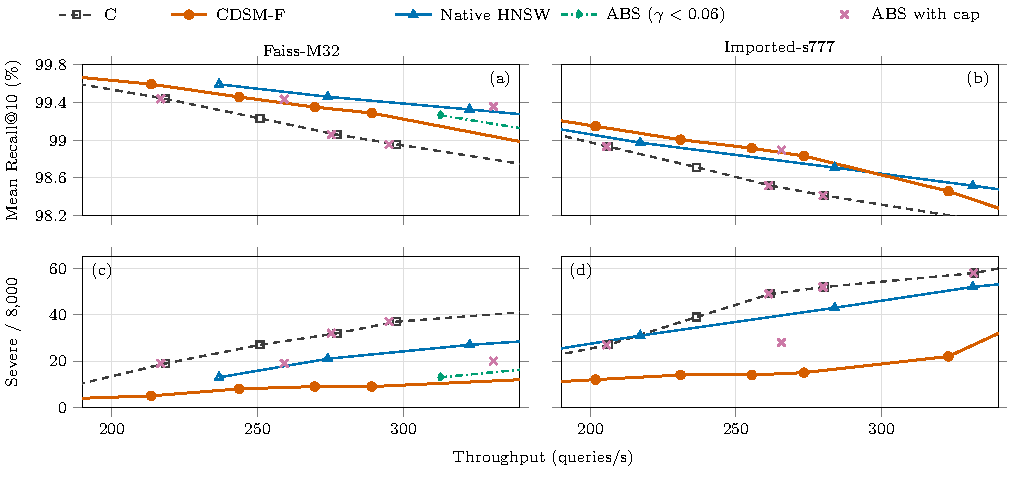
\includegraphics[width=\textwidth]{native-tradeoff.pdf}
\Description{Four panels enlarge the high-recall, 190 to 340 queries per second region on two T2I graphs for C, CDSM-F, native HNSW, ABS, and capped ABS.}
\caption{High-recall operating region on Faiss M32 and imported seed 777. This is an axis zoom of the complete measured grid, with no Pareto filtering. Uncapped ABS uses $\gamma<0.06$; ABS\_CAP retains its independent grid. All timing belongs to the earlier native wave. Figure~\ref{fig:nativefull} retains the full range; Table~\ref{tab:native} gives four-graph selected points.}
\label{fig:native}
\end{figure*}

At those selected points, F has fewer severe failures than native Faiss on all four graphs, with adjusted evidence on seeds 777/1234 in the original 28-test family. Mean recall is higher on the imported graphs and lower on Faiss M32; QPS is lower everywhere. Restricting uncapped ABS retrospectively to $\gamma<0.06$ selects 0.058 from its recorded development grid on every graph. F then has higher recall, fewer severe failures, and shorter p99 than ABS, but lower QPS. Earlier unrestricted-ABS tests are not transferred to this comparison.

The complete native grid also contains joint quality--time advantages. We match every native point to the fastest measured F point with no lower mean recall and no more severe failures, and perform the reverse match; all unmatched points remain in the artifact. On seed 777, native ef 1,280 versus F at 11,264 gives recall 98.97375\% versus 99.00500\%, severe counts 31 versus 14, and QPS 217.18 versus 231.04 ($+6.38\%$). The p99 query-median latency falls from 6.193 to 5.411\,ms. This is a local advantage in an exposed evaluation grid, not a development-selected deployment choice, an equal-work comparison, or evidence of whole-grid dominance.

ABS\_CAP offers a further tradeoff, often with higher mean recall or speed than F but an equal or larger severe count. Its selected cap is 12,800, versus F's 10,240; actual work can stop early. C's p99 is already close to F's (4.596--4.926 versus 4.578--4.877\,ms across these graphs). Consequently, the hard cap explains part of the tail-time advantage over uncapped ABS; it cannot all be attributed to scouts.

\paragraph{Why disclose a restricted ABS range?}
The current uncapped range $\gamma<0.06$ was adopted after inspecting costs, rather than preregistered as a universal cutoff. Table~\ref{tab:abscost} retains the cost evidence. On LAION, $\gamma=0.06$ averages 74,096 distance evaluations and 44.969\,ms; $\gamma=0.09$ averages 352,969 and 271.292\,ms. The latter's p99 approaches 1.27\,s despite normal distance-rule termination. These points are cost context outside the current ranking, not equal-resource competitors to F at 10,240. Growth depends on the workload and already occurs below 0.06; the parameter bound itself is not a resource guarantee. We therefore report actual work, caps, and observed tail time separately, without introducing a post-hoc service deadline.

\begin{table}[t]
\centering
\caption{LAION ABS cost context. Means average three graphs; p99 ranges span their 800-query timing subsets. Rows $\gamma\geq0.06$ are excluded from current ranking.}
\label{tab:abscost}
\small
\begin{tabular}{@{}rrrr@{}}
\toprule
$\gamma$ & Mean DC & Mean ms & p99 ms \\
\midrule
0.030 & 4,944 & 2.623 & 14.5--16.1 \\
0.050 & 33,744 & 19.203 & 170.5--174.5 \\
0.058 & 64,038 & 38.418 & 357.9--360.7 \\
0.060 & 74,096 & 44.969 & 417.5--422.9 \\
0.090 & 352,969 & 271.292 & 1263.2--1276.6 \\
\bottomrule
\end{tabular}
\end{table}


\subsection{Frozen transfer to LAION and WebVid}\label{sec:transfer}
Frozen binaries, settings, and analysis transfer without re-selection. All three caps and both family allowances match actual work; repeated C/F quality agrees with prior measurements. These cohorts were previously used.

\begin{table*}[t]
\centering
\caption{Frozen transfer at 10,240 evaluations. Recall and mean time are equal-weight graph averages; severe counts retain seeds 42/777/1234 separately. The p99 range spans graph-level p99 values, not pooled query latencies.}
\label{tab:transfer}
\small
\begin{tabular}{@{}llrrrr@{}}
\toprule
Dataset & Method & Recall (\%) & Severe / 8,000 & Mean (ms) & p99 range (ms) \\
\midrule
LAION & C & 95.3871 & 35 / 33 / 31 & 5.531 & 6.809--6.848 \\
LAION & F & 95.2525 & 33 / 33 / 35 & 5.609 & 6.800--6.885 \\
LAION & FANNG & 95.3875 & 35 / 32 / 32 & 9.867 & 13.483--13.784 \\
WEBVID & C & 97.2738 & 20 / 25 / 18 & 5.603 & 6.890--6.943 \\
WEBVID & F & 97.1996 & 21 / 20 / 19 & 5.667 & 6.803--6.821 \\
WEBVID & FANNG & 97.2771 & 20 / 24 / 18 & 10.025 & 13.349--13.421 \\
\bottomrule
\end{tabular}
\end{table*}


At 10,240, F lowers mean recall on every graph (Table~\ref{tab:transfer}): LAION changes are $-0.16750/-0.11000/-0.12625$ percentage points; WebVid changes are $-0.09375/-0.05375/-0.07500$. Rescues/harms are 3/1, 3/3, 2/6 and 4/5, 6/1, 3/4, respectively; more queries lose hits than gain them everywhere. QPS decreases by 1.82/1.06/1.28\% and 1.12/0.89/1.37\%; five of six differences are within tolerance. F is faster than FANNG but has lower mean recall; none of the primary severe tests passes Holm.

At the family primary allowance, WebVid's C/F severe counts are 24/23, 27/21, and 23/23, with QPS decreases of 1.015--1.127\% and lower mean recall. Across both datasets and allowances, F's mean recall is lower than C in all twelve configurations; each extension is lower than F in all twelve. KEEP matches DIVERSE's severe counts, and E64\_RAW lowers mean recall versus KEEP everywhere. Neither dataset has an adjacent primary contrast passing Holm.

As a secondary outcome, F lowers zero failures in eight of WebVid's nine absolute cells (one tie); LAION has six decreases, two ties, and one increase. Some family configurations instead increase zero failures. These outcomes do not replace the primary severe endpoint. Transfer supplies no online rule predicting beneficial queries.

\subsection{Applicability from a T2I reference configuration}\label{sec:scope}
The settings in Table~\ref{tab:parameters} define a reference, not a universal optimum. T2I evidence covers previously unused queries, four graph constructions, three absolute budgets from 8,192 to 12,800, and two $p+E$ allowances. Table~\ref{tab:fixed} adds a current-implementation depth check at 10,240: limits 200, 400, and 800 all improve mean recall and severe counts over C on every graph. At 200, recall gains are 0.188--0.309 percentage points, severe counts are 11/23/21/24, and QPS decreases by only 0.07--0.77\%, within practical tolerance. At 800, severe counts are 8/20/14/20, while mean recall rises versus F on two graphs and falls on two. These descriptive results support neighboring configurations without changing the frozen primary F or establishing pure entrance-count superiority. Appendix~\ref{app:secondary} separates the older Java depth evidence.

Applying the same settings to another embedding collection is a testable extrapolation. LAION and WebVid show that the cross-modal label alone does not predict a joint quality gain: some tail outcomes improve while mean recall falls. The present method is therefore useful on the demonstrated T2I workloads, with measured external boundaries. Larger collections, different graph families, and automatic selection of beneficial queries remain unestablished; the negative transfer does not justify claiming that an untested parameter scaling would repair it.

\section{Why Retain Unfinished Exploration?}\label{sec:explanation}
\subsection{Local exploration needs room to develop}\label{sec:ablation}
A full-cohort factorial experiment varies scout admission and distance stopping on the 7,999-query, three-graph cohort. It is a retrospective mechanism extension after that cohort was exposed, with no new formal timing. Every policy uses the same $p+6{,}400$ actual distance work per event; each scout retains its 400-evaluation cap, including upper descent. L denotes strict local admission. GLOBAL stops against the main collector's threshold, LOCAL against the scout's local threshold, and NONE removes distance-based early stopping while retaining the cap and eligibility rules.

\begin{table}[t]
\centering
\caption{Scout stopping rules on 7,999 queries and three graphs (23,997 events). All policies match actual work per event. Bottom DC is mean new bottom-layer scoring in the scout phase; it excludes upper descent.}
\label{tab:stop}
\small
\begin{tabular}{@{}lrrrr@{}}
\toprule
Policy & Recall (\%) & Severe & Zero & Bottom DC \\
\midrule
C & 99.02654 & 65 & 25 & 0.00 \\
L\_GLOBAL & 99.09739 & 46 & 15 & 0.36 \\
L\_LOCAL (F) & 99.18240 & 26 & 10 & 1098.68 \\
L\_NONE & 99.17031 & 24 & 10 & 1342.70 \\
\bottomrule
\end{tabular}
\end{table}


Table~\ref{tab:stop} shows why immediately applying a mature global threshold can curtail a new route. L\_GLOBAL spends only 0.36 new bottom-layer distances per event across its scouts, compared with 1,098.68 for F. Their mean upper-descent costs are similar (254.86 and 253.86). F raises recall and reduces severe events from 46 to 26, with 22 rescues and two harms. The risk reduction is 0.08334 percentage points, with a descriptive query-cluster 95\% interval of [0.03750, 0.13335]. Unused scout work goes to final continuation, so the intervention tests a complete allocation policy, not stopping at equal scout expenditure.

L\_NONE has 24 severe events, two fewer than F, but slightly lower mean recall. Thus the local stopping rule is not uniquely effective or best on every metric. Allowing all discovered neighbors into the scout queue (A\_LOCAL) instead of strict local admission produces the same scoring paths and returned sets as F on all 23,997 events. A constructed distance-tie example distinguishes these rules; their observed agreement is not a theorem. The full factorial results in Appendix~\ref{app:factorial} prevent attributing the benefit to an admission filter unsupported by the ablation.

\subsection{Answers and continuation opportunities differ}
We use selected execution interventions to explain the design after establishing its overall effect. An earlier study selected 55 rescued and five harmed T2I events. For 22 of the 55 rescues, combining \emph{all} candidates scored by a complete C search with all candidates scored by scouts fails to reproduce the rescue. This is stronger than combining returned top-ten lists: it retains every scored candidate, yet lacks later discoveries made during F's continuation.

The strengthened union control uses 13,893.08 evaluations on average, exceeding F's 12,800. It tests candidate sufficiency, not equal-work performance. A separate intervention retains executable continuation states and compares six schedules at exactly 12,800 evaluations per event. Splitting remaining continuation 25\% or 50\% to the C state and running C before F preserves all 22 later rescues. Running F before C preserves 21 and 18, respectively. Thus feedback can enable later discoveries, while execution order still determines which opportunities are realized. These diagnostic schedules differ from F's production merge and do not prove that every operation is necessary.

The selected events do not estimate mechanism frequency in the full population. Search order, shared scores, visitation, and continuation state interact. The inference is that preserving an opportunity for subsequent discovery can matter, not that a uniquely identified queue or edge explains every improvement.

\subsection{Scouts spend opportunities on the original route}
Retaining more state does not refund the cost of exploration. We examine the recorded C/F prefixes while preserving the full original scout prefix and charging overlapping distance work once. Restoring five hits requires at least 13,859, 13,298, and 13,268 evaluations in three of the five harmed events. Each exceeds the original 12,800 allowance. Reallocating work among those recorded prefixes cannot eliminate these harms within that allowance.

This is a restricted-family result, not a lower bound for arbitrary graph searches. A different entrance, expansion order, scout requirement, or larger allowance may change the outcome. Its design implication is concrete: alternative exploration must be judged against the useful main-route work it displaces. The LAION and WebVid outcomes demonstrate why keeping more scout state or adding a selection stage is insufficient by itself.

\section{Related Work}
\label{sec:related}



\paragraph{Search organization on existing graphs.}
HNSW combines hierarchical navigation and proximity-graph search~\cite{hnsw}; Faiss and Lucene implement it~\cite{faiss,lucene}. CDSM changes query allocation on existing edges. Local queues, visited state, and resumed expansion have precedents; the contribution is the specific bounded-exploration and reintegration policy.

FANNG retains unexplored edges and backtracks under a distance budget~\cite{fanng}. CDSM additionally gives backup entrances local exploration before returning unfinished work. Our control adapts FANNG search, excluding native construction and system performance.

\paragraph{Multiple paths and resumed execution.}
iQAN uses multiple paths, local queues, shared visitation, and adaptive synchronization for intra-query parallelism~\cite{iqan}. Its feedback can affect global expansion, so that principle is not unique to CDSM. Table~\ref{tab:semantics} identifies our distinction: upper-entrance exploration after a main prefix, explicit local allowances, and unfinished-state integration into one budgeted continuation. The difference concerns exploration's source, timing, allocation, and integration, beyond sequential versus parallel execution. MEP does not reproduce iQAN.

pgvector 0.8.0 retains discarded candidates and visitation to resume HNSW scans~\cite{pgvector}. CDSM first generates additional work through bounded backup exploration; resumption alone is not its novelty claim.

\paragraph{Choosing entrances.}
Oguri and Matsui select query-dependent starting points from representatives obtained by clustering~\cite{oguri}. GATE extracts hubs and learns a navigation structure using graph topology and query information~\cite{gate}. These approaches improve where exploration begins; CDSM specifies how alternative exploration and retained main-search work share a limited budget. The design dimensions are complementary, although their interaction requires evaluation. Our fixed entrance table and paid-selection extensions are not implementations of either selector, and original CDSM does not learn entrance quality.

\paragraph{Budget, workload, and quality.}
Adaptive Beam Search changes the distance-based termination rule and relates its guarantees to graph navigability~\cite{abs}. CDSM instead budgets exploratory and continuation work; its accounting limit does not imply a recall guarantee. Steiner-Hardness demonstrates the importance of graph-dependent query difficulty~\cite{steiner}, motivating evaluation beyond a workload average without making severe-failure measurement itself novel. RoarGraph addresses cross-modal workloads through query-guided index construction~\cite{roargraph}, whereas CDSM reuses existing edges. Our frozen-policy transfer results delimit its benefits: the T2I improvements do not establish a general advantage on LAION or WebVid. State interventions explain the method's behavior while its measured search-policy benefits remain the main contribution.

\section{Conclusion}
CDSM redirects main-search continuation through bounded local exploration and shared unfinished work. On T2I, its original four-scout policy improves mean recall and severe-failure counts over direct continuation at equal actual distance work. Expanded multi-entry and frontier controls establish additional average-quality benefits at the primary budget, while exposing competing tail-quality choices. Identified operating points also improve quality and throughput over giving continuation 10\% more computation. Local-stop ablations explain how exploration supports later discovery; paid selection and frozen LAION/WebVid transfer delimit applicability. CDSM is a concrete search policy with demonstrated benefits, measured costs, and a reproducible resource contract.

\appendix
\section{Execution and Evaluation Details}\label{app:details}
% Queue the wide appendix table early enough to precede the references.
\begin{table*}[t]
\centering
\caption{Secondary family allowance $E=6{,}400$ on all datasets. Mean recall (R) is a graph average in percent; severe counts (S) remain per graph, each out of 8,000. These are descriptive secondary endpoints.}
\label{tab:secondary}
\small
\begin{tabular}{@{}lrrrrrr@{}}
\toprule
Method & T2I R & T2I S & LAION R & LAION S & WebVid R & WebVid S \\
\midrule
C & 99.0666 & 19 / 22 / 27 / 29 & 96.0179 & 25 / 18 / 23 & 97.7004 & 16 / 15 / 12 \\
FANNG & 99.0691 & 19 / 21 / 27 / 28 & 96.0154 & 25 / 18 / 24 & 97.7013 & 16 / 15 / 12 \\
F & 99.2391 & 5 / 11 / 12 / 15 & 95.9171 & 25 / 18 / 23 & 97.6771 & 14 / 16 / 11 \\
SCORE & 99.2694 & 2 / 7 / 12 / 13 & 95.8404 & 24 / 21 / 24 & 97.6150 & 15 / 17 / 12 \\
DIVERSE & 99.2844 & 3 / 6 / 11 / 9 & 95.8204 & 25 / 21 / 25 & 97.6150 & 14 / 17 / 11 \\
KEEP & 99.2837 & 3 / 6 / 10 / 9 & 95.8208 & 25 / 21 / 25 & 97.6150 & 14 / 17 / 11 \\
E64\_RAW & 99.2884 & 2 / 7 / 8 / 9 & 95.7812 & 27 / 21 / 26 & 97.5938 & 14 / 17 / 11 \\
\bottomrule
\end{tabular}
\end{table*}

\begin{table*}[t]
\centering
\caption{Primary transfer allowance $E=3{,}200$: graph-average recall R (\%) and per-graph severe counts S / 8,000, in seed order 42/777/1234.}
\label{tab:transferfamily}
\small
\begin{tabular}{@{}lrrrr@{}}
\toprule
Method & LAION R & LAION S & WebVid R & WebVid S \\
\midrule
C & 95.2017 & 37 / 36 / 35 & 97.1383 & 24 / 27 / 23 \\
FANNG & 95.2037 & 37 / 35 / 36 & 97.1433 & 24 / 26 / 23 \\
F & 95.0229 & 37 / 39 / 37 & 97.0187 & 23 / 21 / 23 \\
SCORE & 94.8825 & 40 / 38 / 45 & 96.8983 & 24 / 25 / 21 \\
DIVERSE & 94.8508 & 41 / 36 / 44 & 96.8937 & 24 / 22 / 19 \\
KEEP & 94.8500 & 41 / 36 / 44 & 96.8933 & 24 / 22 / 19 \\
E64\_RAW & 94.7975 & 42 / 35 / 45 & 96.8408 & 24 / 22 / 19 \\
\bottomrule
\end{tabular}
\end{table*}

\begin{figure*}[t]
\centering
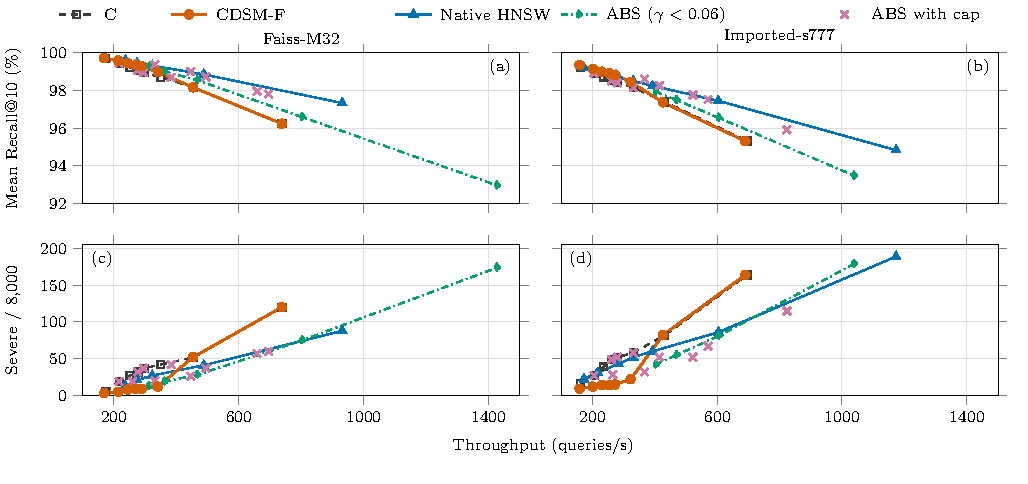
\includegraphics[width=\textwidth]{native-full.pdf}
\Description{Full measured parameter ranges on Faiss M32 and imported seed 777 show mean recall and severe counts against throughput for five search methods, without Pareto filtering.}
\caption{Full range corresponding to Figure~\ref{fig:native}, using the same data and timing wave. Every allowed point is retained, including dominated points. ABS\_CAP is a scatter series because both its cap and stopping parameter vary. The source package includes all four graphs' full summaries.}
\label{fig:nativefull}
\end{figure*}
\begin{table*}[t]
\centering
\caption{Four-graph points selected by development mean time $\leq4$\,ms. R is mean recall; S is severe events / 8,000. Uncapped ABS is restricted retrospectively to $\gamma<0.06$. All values belong to the earlier native wave, without equal-work or equal-time claims.}
\label{tab:native}
\small
\begin{tabular}{@{}llrrrr@{}}
\toprule
Graph & Metric & Native & F & ABS & ABS\_CAP \\
\midrule
Faiss M32 & R (\%) / S & 99.46125 / 21 & 99.35125 / 9 & 99.26500 / 13 & 99.43625 / 19 \\
 & QPS / p99 ms & 274.10 / 5.337 & 269.64 / 4.578 & 312.82 / 20.910 & 259.20 / 5.857 \\
Imported 42 & R (\%) / S & 98.76500 / 39 & 98.84125 / 22 & 98.00500 / 36 & 98.98875 / 22 \\
 & QPS / p99 ms & 284.94 / 4.822 & 255.10 / 4.877 & 405.98 / 16.949 & 266.15 / 6.141 \\
Imported 777 & R (\%) / S & 98.70875 / 43 & 98.91500 / 14 & 97.93375 / 42 & 98.89500 / 28 \\
 & QPS / p99 ms & 283.93 / 4.812 & 255.44 / 4.870 & 403.68 / 16.940 & 265.73 / 6.157 \\
Imported 1234 & R (\%) / S & 98.73125 / 42 & 98.81000 / 20 & 97.92375 / 44 & 98.87000 / 30 \\
 & QPS / p99 ms & 283.69 / 4.804 & 254.48 / 4.877 & 400.13 / 17.577 & 264.61 / 6.151 \\
\bottomrule
\end{tabular}
\end{table*}


\subsection{Execution details}
\label{app:execution}

For a native graph, the entrance pool concatenates node IDs from successive
upper layers, in increasing layer and ID order. A node on multiple upper
layers occurs repeatedly in the pool. A Java-compatible pseudorandom
generator seeded by the graph's node count samples that pool, rejecting
already accepted IDs until 64 distinct nodes (or all eligible nodes) have
been accepted. First acceptance determines table order. Imported graphs
retain their saved table. The order is independent of the query; no
recall or rescue label determines it.

Queues and answers use $(\hbox{distance},\hbox{node ID})$ order.
Admission compares $d<\tau$ before updating the local threshold;
local stopping compares $d>\tau$ between expansions.
An earlier admission may reach or exceed the tightened threshold, so
these tie rules differ. Initial stopping uses $\geq(1+\gamma)^2\tau_A$;
final continuation disables it.

Score validity, bottom-layer discovery, adjacency opening, and completion
are separate states. An upper-scored node can enter bottom traversal
without another evaluation. An already discovered neighbor is skipped
while the source cursor advances. Completion requires processing all
neighbors; stale queue references to completed nodes are then discarded.

F merges active, deferred, and current scout work into the main active
queue without replacing the main current node. Shared bottom cursors
preserve partial scans. F does not save an upper cursor if descent
exhausts its allowance: no bottom seed is installed, but computed scores
still contribute to the answer collector.

\subsection{Admission and stopping factorial}\label{app:factorial}
The six scout variants cross strict local admission (L) or all-neighbor
admission (A) with LOCAL, GLOBAL, or NONE distance stopping. Under LOCAL,
A and L have identical scored paths and answers on all 23,997 events;
the same agreement holds under GLOBAL. Under NONE, A returns 99.17698\%
mean recall, 24 severe events, and nine zero events, compared with
99.17031\%, 24, and ten for L. The unchanged severe count contains one
rescue and one harm. These retrospective results have descriptive
query-cluster intervals, not multiplicity-adjusted confirmation or new
timing. The original F policy is L\_LOCAL throughout the paper.

\subsection{Recall distribution and threshold checks}\label{app:thresholds}
\begin{table}[t]
\centering
\caption{Recall-tail sensitivity of C versus F on the 7,999-query cohort (23,997 graph--query events). Counts are descriptive; threshold 5 is the original severe endpoint.}
\label{tab:thresholds}
\small
\begin{tabular}{@{}rrrr@{}}
\toprule
Hits below & C & F & Rescue / harm \\
\midrule
1 & 25 & 10 & 17 / 2 \\
3 & 45 & 18 & 28 / 1 \\
5 & 65 & 26 & 41 / 2 \\
7 & 90 & 40 & 55 / 5 \\
9 & 280 & 218 & 95 / 33 \\
10 & 1542 & 1516 & 145 / 119 \\
\bottomrule
\end{tabular}
\end{table}

Table~\ref{tab:thresholds} recomputes saved hits from all 23,997 matched
pairs and checks the frozen totals. Counts are events, not independent
queries. Five remains the severe threshold; other cutoffs are descriptive,
not additional significance tests. The artifact retains the complete
zero-to-ten hit histograms and their source records.

\subsection{Workspaces and reproducibility}\label{app:repro}
The C++ executor allocates per-node score, query stamp, upper-descent stamp, adjacency-position, adjacency-end, and flag arrays. With 4-byte floats and integers and 1-byte flags, their payload is $21N$ bytes: 21.0\,MB (20.03\,MiB) for a million nodes. C and F instantiate the same workspace, so this is \emph{not} F's incremental memory over C. Dynamic heaps, adjacency storage, touched lists, vector capacity, objects, and the index are additional. F's local queues create dynamic work; static accounting does not establish peak RSS or concurrent-query costs. The FANNG sorted adjacency view is also separate preprocessing and storage, not charged as query distances.

Input hashes bind the vectors, graph, canonical-ID map, entrance table, ground truth, query manifest, and budget manifest. The frozen source and binaries precede each evaluation. New comparisons audit every actual score count and repeated output, with engineering checks against archived execution paths. Quality runs and formal timing are separated. A global experiment lock and serialized timing avoid concurrent timing by this project; these are controlled process measurements, not a production-service workload.

The LAION subset uses image embeddings from the first LAION-400M embedding shard and text queries from another shard~\cite{laionembeddings}. WebVid uses a fixed CLIP-WebVid video-embedding subset with separately encoded caption queries~\cite{clipwebvid,clip}. Exact subsets, query provenance, and executable versions are retained in the source manifests. No benefit is inferred simply from either dataset being cross-modal. The repeated transfer cohorts were already exposed in the preceding dataset evaluations.

\subsection{Secondary budgets and statistical scope}\label{app:secondary}
Tables~\ref{tab:secondary} and~\ref{tab:transferfamily} retain all seven methods at the secondary allowance and the transfer primary allowance. Each severe-count component is out of 8,000 queries; graph order is Faiss M32 then seeds 42/777/1234 for T2I, and seeds 42/777/1234 for transfer. Averages across graphs are descriptive because query identities repeat. The source package retains every primary and secondary per-graph metric and timing round; none is filtered to a Pareto frontier before presentation.

The earlier C/F server study used 28 comparisons; FANNG used four and the extension study twenty. Each transfer dataset separately used three fixed-cap and fifteen family tests, with none passing Holm. The latest twelve-test MEP/FRONTIER family remains separate. These families do not provide a pooled cross-dataset guarantee. The 7,999-query F/C contrast is descriptive because its primary test concerned a conditional policy; the 1,600-query MEP intervals are unadjusted. Absence of significance does not establish equality.

\paragraph{Historical parameter evidence.}
Table~\ref{tab:depthhistory} explains why 400 is a retained engineering compromise. With four 100-evaluation routes, 2,161 of 24,000 route attempts exhaust their allowance before bottom seeding; none does so at 400. Increasing 400 to 1,600 raises final mean recall by only 0.01 percentage points. This retrospective Java evidence is not a selection protocol for the current C++ experiment. It also does not isolate a pure entrance-count advantage: equal total work does not equalize actual scout expenditure.

\begin{table}[t]
\centering
\caption{Historical depth development: 2,000 T2I queries, three Lucene graphs, Java COSINE, $p+6{,}400$ actual work. $m/s$: maximum routes / per-route limit. $U$: routes exhausting their limit before bottom seeding (\%); S: severe events / 6,000. These are separate from the C++ results in Table~\ref{tab:fixed}.}
\label{tab:depthhistory}
\small
\begin{tabular}{@{}lrrrr@{}}
\toprule
$m/s$ & Scout DC & $U$ (\%) & Recall (\%) & S \\
\midrule
1/100 & 99.98 & 8.88 & 98.8350 & 22 \\
1/400 & 341.23 & 0.00 & 98.9117 & 18 \\
1/1600 & 382.64 & 0.00 & 98.9117 & 18 \\
4/100 & 399.95 & 9.00 & 98.9167 & 17 \\
4/400 & 1349.55 & 0.00 & 99.0067 & 13 \\
4/1600 & 1519.81 & 0.00 & 99.0167 & 12 \\
\bottomrule
\end{tabular}
\end{table}


\subsection{Complete native operating range}\label{app:nativegrid}

The native choices are ef 896 on Faiss M32 and ef 1,024 on the imported
graphs; F selects cap 10,240. Restricted ABS selects $\gamma=0.058$;
ABS\_CAP selects $\gamma=0.1$, cap 12,800. The ABS restriction is
retrospective and old tests for unrestricted selections are not reused.
Figure~\ref{fig:nativefull} includes the measured grid, while
Table~\ref{tab:native} reports the development-selected comparison.

The artifact rebuilds tables, vector figures, and this manuscript from
bundled frozen summaries and the retained per-event hit records used for
threshold analysis. Rebuilding the paper does not rerun ANN search.
Full experimental reproduction additionally requires the indexed vectors,
query sets, ground truth, graph files, binaries, and execution environment
identified in the manifests; these large inputs are not all bundled.

\balance
\bibliographystyle{ACM-Reference-Format}
\bibliography{references}
\end{document}
